\documentclass{article}
\usepackage[margin=1.5cm,bottom=2cm]{geometry}
\usepackage{fancyhdr}
\usepackage{graphicx}
\usepackage[section]{placeins}
\pagestyle{fancy}
\usepackage{amsmath}

\begin{document}
\fancyhead[L]{ 
\includegraphics[width=2cm]{au_logo.png} }
\fancyhead[R]{PHYS 2240: General Physics II}
\fancyfoot[C]{\thepage}
\vspace*{0cm}
\begin{center}
	{\LARGE \textbf{Lab 6}}\\
	\vspace{.25cm}
	{\Large Centripetal Acceleration}
	%\vspace{0.25cm}
	%{\Large Due: Friday, September 4}
\end{center}

\section*{Introduction}
When a mass moves in a circle at constant speed, its change in momentum is directed inward, toward the center of the circular path. The magnitude of the change in momentum is:
\begin{equation}
	\left|\frac{d\vec{p}}{dt}\right|_\perp=m\frac{v^2}{r}
\end{equation}
Our experiment will attempt to confirm this relationship.

\section*{Overview}
In this experiment, you will rotate a mass in a circle and measure the force two different ways. The experimental apparatus is shown in Figure \ref{exp}. It works like this: the hanging mass is initially given some velocity by spinning the vertical shaft. The mass is attached to the vertical shaft via a spring and a tether attached to a horizontal cross arm (see Figure \ref{exp}). The free body diagram during this rotation is shown in Figure \ref{fbd}.

Since $\left|\frac{d\vec{p}}{dt}\right|_\perp=m\frac{v^2}{r}$ and $|\vec{F}_\mathrm{net}|_\perp=k|s|$, spinning the mass with higher speed will stretch the spring and cause the mass to rotate with a greater radius of curvature.

If the mass rotates at a constant radius $r$, and you rotate it $f$ times per second, then its speed is:
\begin{equation}
	v=2\pi rf
\end{equation}
\section*{Details}
For each trial of this lab, you will:
\begin{enumerate}
	\item Choose a radius of curvature (using the radius indicator in Figure \ref{exp})
	\item Rotate the vertical shaft with increasing frequency, until the radius of curvature of the mass matches the radius you chose in step 1. Measure this frequency.
	\item Using your measured value of $r$ and $f$, calculate $v$ and $F_\mathrm{spring}=m\frac{v^2}{r}$. This is your \textit{theoretical} value for force.
	\item Test your result from step 3 by attaching a hanging mass to the rotating mass to pull it outwards. Continue adding mass to the hanging mass until the rotating mass reaches the radius indicator. This will be your experimental force ($mg$).
\end{enumerate}
Repeat these measurements for 5 different values of $r$, and record your values in the table.
\begin{figure}[ht!]
	\centering
	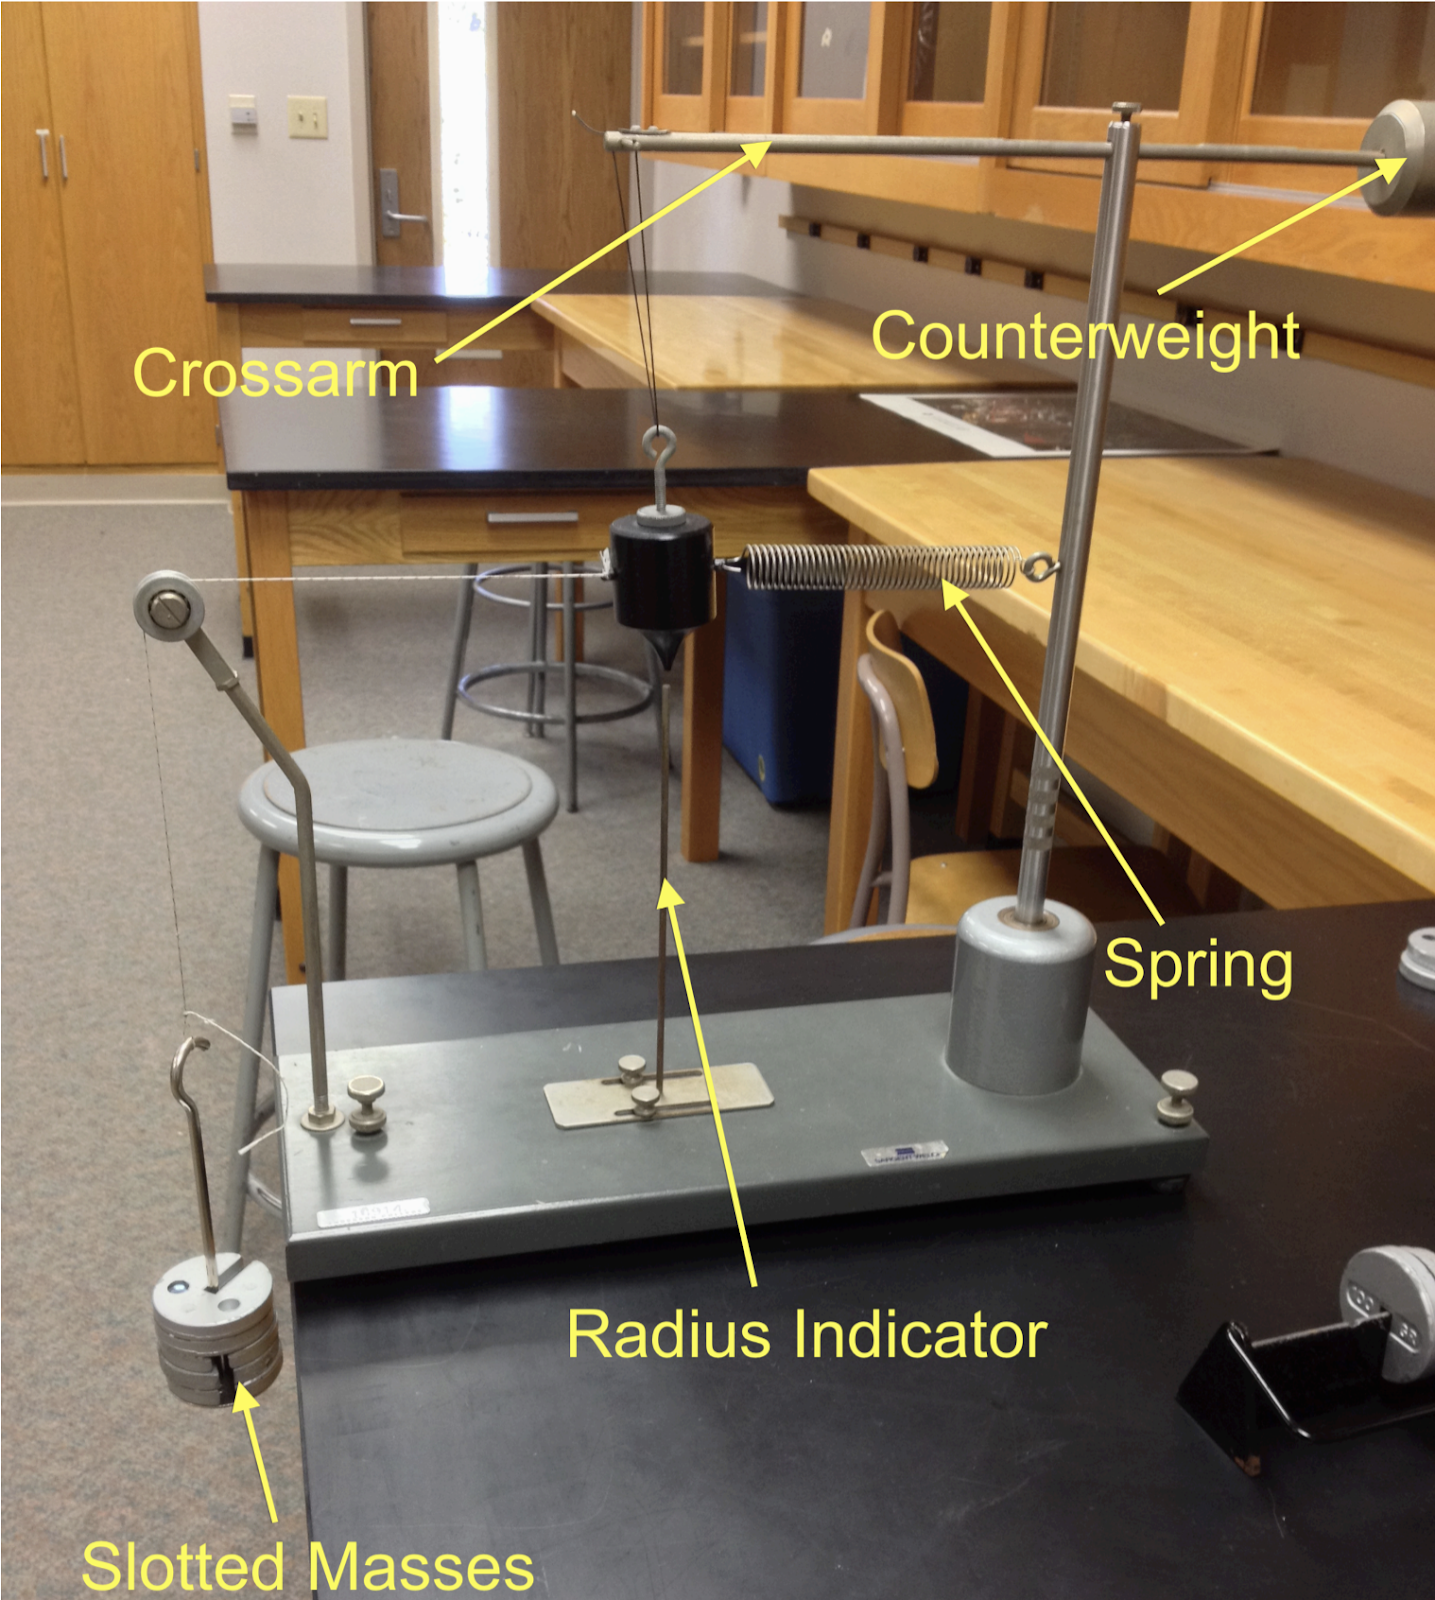
\includegraphics[width=0.4\textwidth]{centripetal.png}
	\caption{The experimental apparatus}
	\label{exp}
\end{figure}

\begin{figure}[ht!]
	\centering
	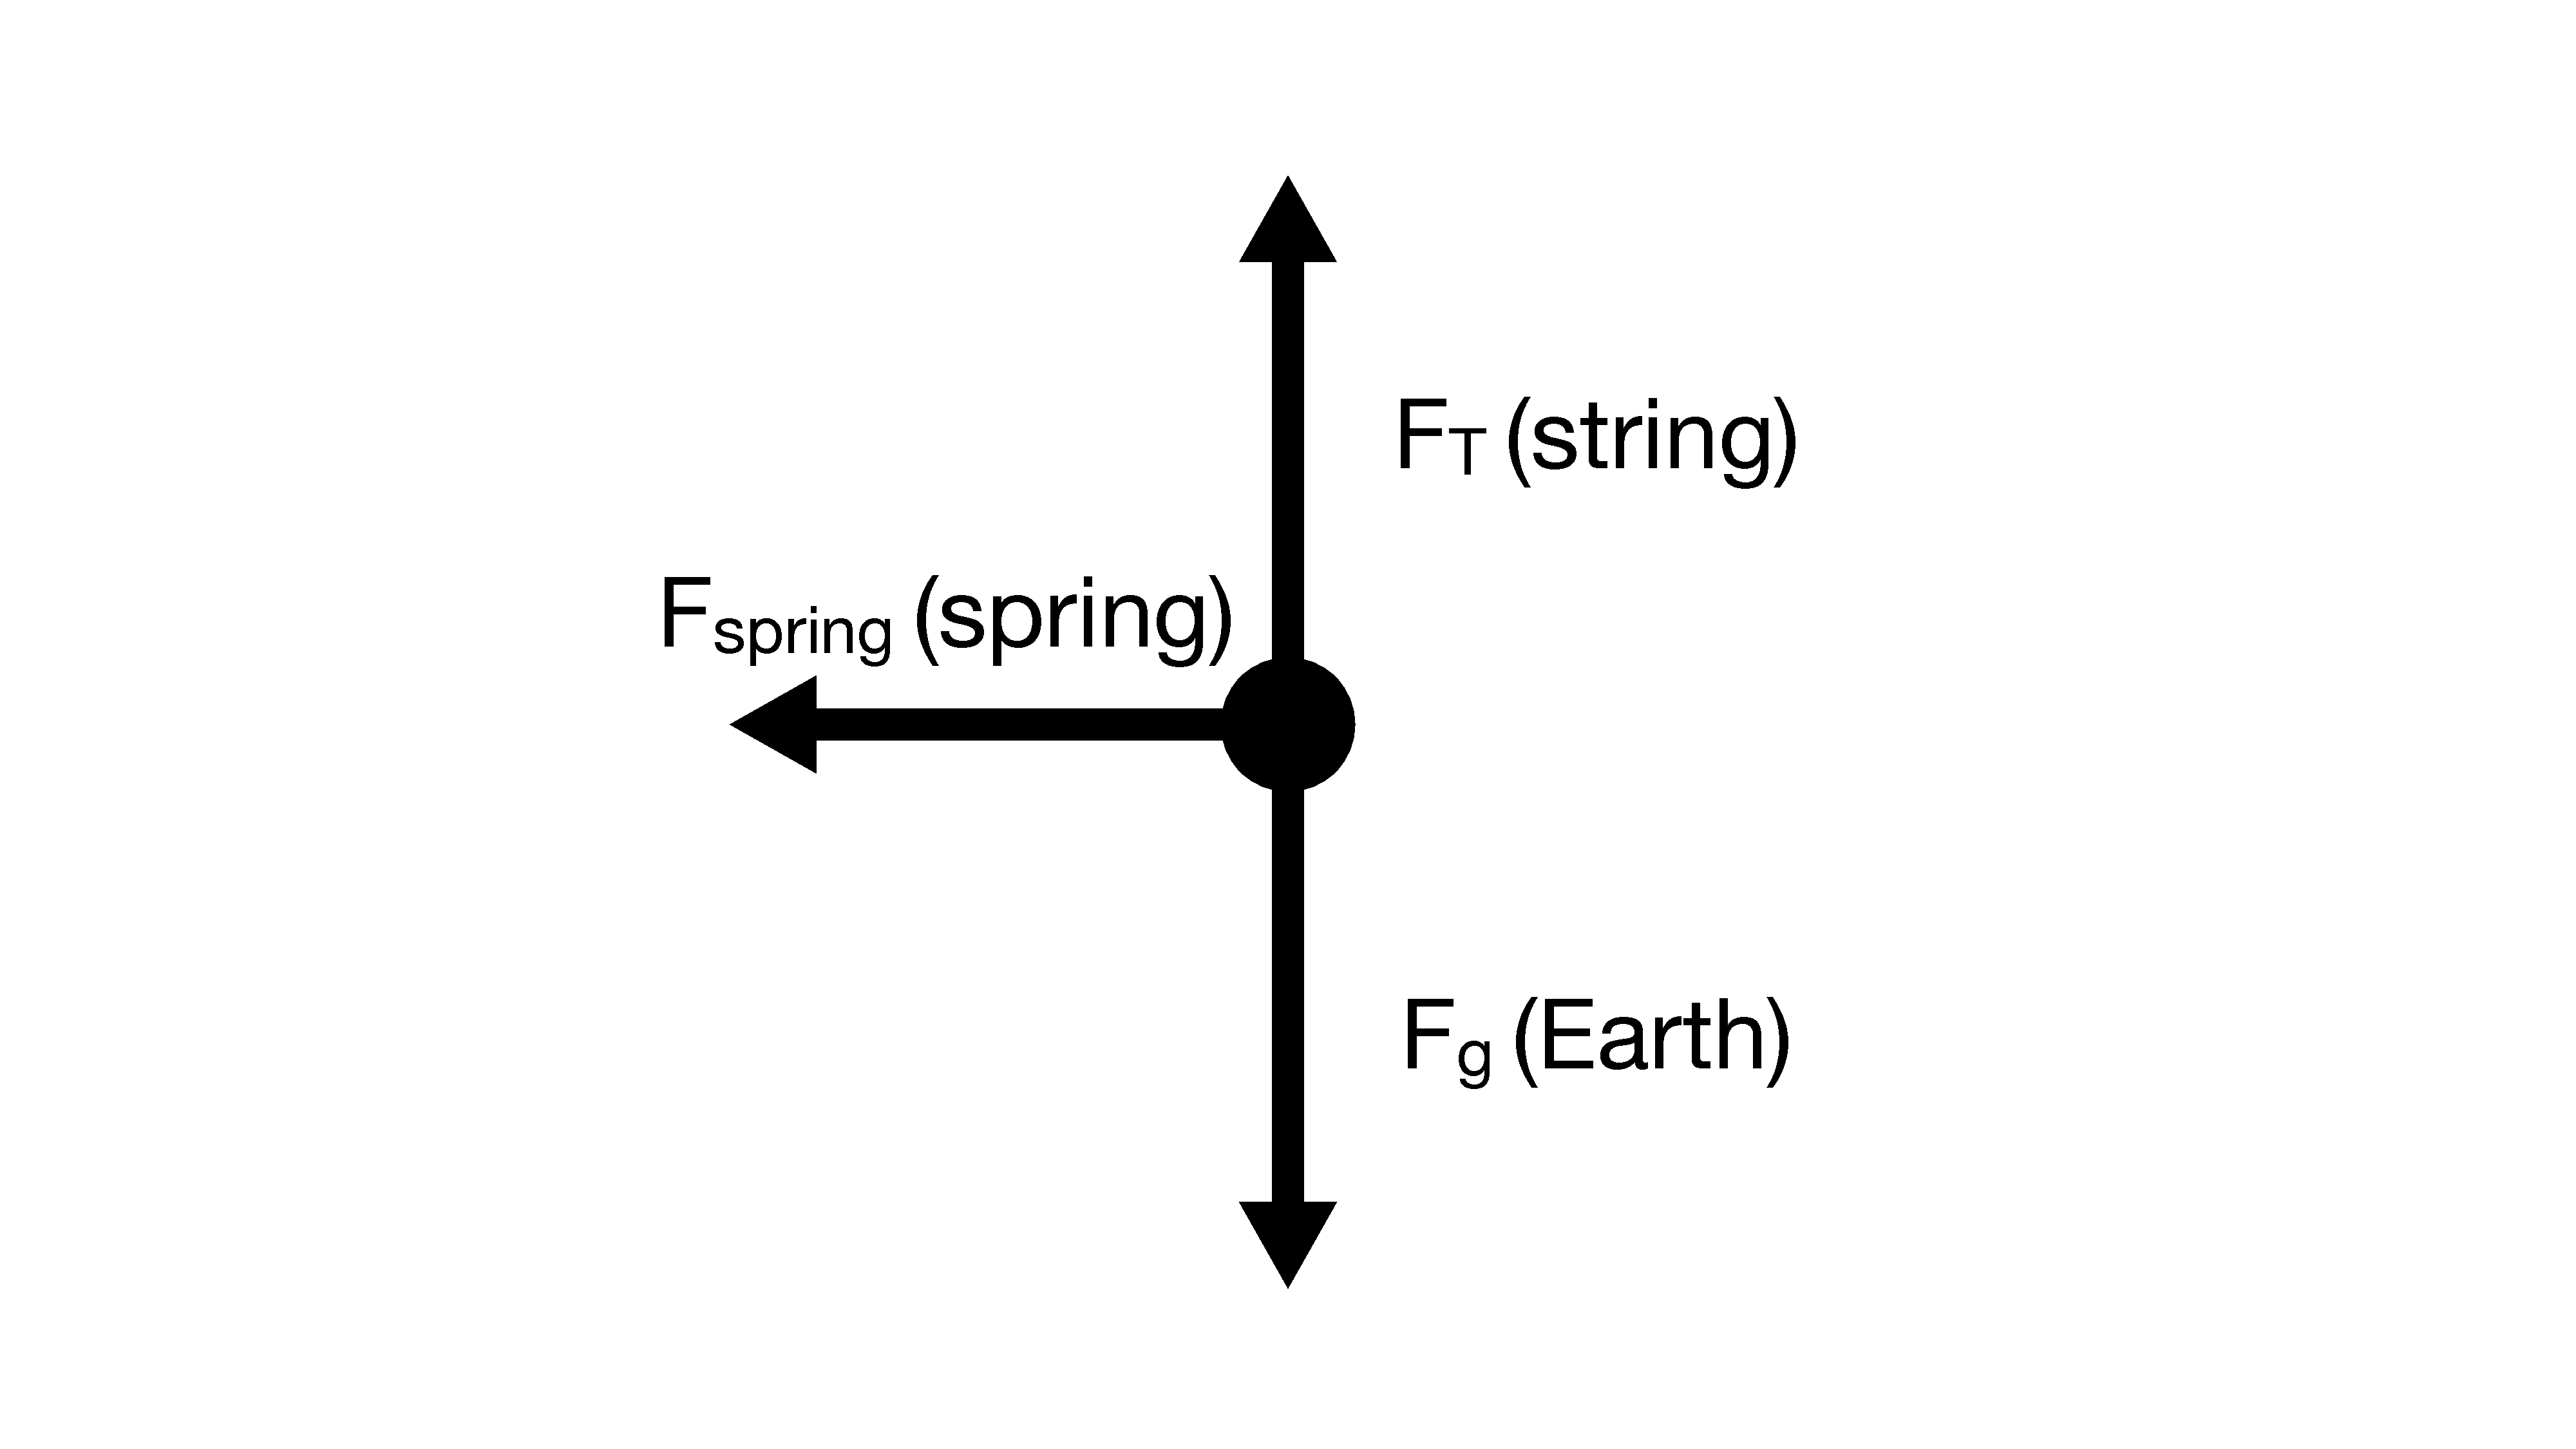
\includegraphics[width=0.4\textwidth]{fbd.pdf}
	\caption{Free body diagram}
	\label{fbd}
\end{figure}

\begin{center}
\begin{tabular}{|c|c|c|c|}
	\hline
	$r$ [m]&$f$ [$s^{-1}$]&$F_\mathrm{theory}$ [N]&$F_\mathrm{exp}$ [N]\\
	\hline
	&&&\\
	\hline
	&&&\\
	\hline
	&&&\\
	\hline
	&&&\\
	\hline
	&&&\\
	\hline
\end{tabular}
\end{center}
\textbf{Keep the following in mind while conducting each trial:}
\begin{itemize}
	\item In order for the free body diagram in Figure \ref{fbd} to be accurate, the upward tensile force must be completely perpendicular (upwards). In order to ensure this, we must adjust the crossarm so that it matches the radius indicator. In any given trial, make sure that the position of the crossarm and radius indicator are positioned such that, when the mass is detached from the spring, it hangs freely exactly over the radius indicator. Therefore, whenever the radius of rotation is changed, the crossarm must be adjusted accordingly.
	\item To find $f$, begin rotating the vertical shaft so that the object begins to revolve.  Accelerate the rotation until the revolving mass begins to pass over the radius indicator. Once the mass is consistently passing over the radius indicator, continue rotating at constant speed.  Measure the amount of time it takes for the object to complete 10-20 revolutions.  The frequency $f$ is then given by: 
	\begin{equation}
		f=\frac{\mathrm{\# \ of\  revolutions}}{\mathrm{time}}
	\end{equation}
\end{itemize}
\section*{Analysis}
\begin{itemize}
	\item Looking at your data, how do $F_\mathrm{theory}$ and $F_\mathrm{exp}$ compare? Do they agree? Why or why not?
	\item Can you use your data to find the spring constant $k$ and relaxed spring length $L_0$?
	\item Centripetal force is an inward (center seeking) radial force. Why, then, does the revolving object move outward?
\end{itemize}
\end{document}